\documentclass{article}

\usepackage[utf8x]{inputenc}
\usepackage[english,russian]{babel}
\usepackage{cmap}
\usepackage{commath}
\usepackage{amsmath}
\usepackage{amsfonts}
\usepackage{mathtools}
\usepackage{amssymb}
\usepackage{parskip}
\usepackage{titling}
\usepackage{color}
\usepackage{hyperref}
\usepackage{cancel}
\usepackage{enumerate}
\usepackage{multicol}
\usepackage{graphicx}
\usepackage{docmute}
\usepackage{titlesec}
\usepackage[font=small,labelfont=bf]{caption}
\usepackage[a4paper, left=2.5cm, right=1.5cm, top=2.5cm, bottom=2.5cm]{geometry}

\graphicspath{ {./images/} }
\setlength{\droptitle}{-3cm}
\hypersetup{ colorlinks=true, linktoc=all, linkcolor=blue }
\pagenumbering{arabic}

\setcounter{secnumdepth}{4}
\setcounter{tocdepth}{4}
\titleformat{\paragraph}
{\normalfont\normalsize\bfseries}{\theparagraph}{1em}{}
\titlespacing*{\paragraph}
{0pt}{3.25ex plus 1ex minus .2ex}{1.5ex plus .2ex}

\begin{document}

\section{Электричество.}
    \subsection{Электростатика.}
        \subsubsection{Два вида заряда.}
            \paragraph{Элементарный электрический заряд, электроны и протоны.}
                Элементарный заряд есть заряд электрона(отрицательный). \(\abs{e} = \abs{p} \approx 1.6 \cdot 10^{-19} \) Кл.

                \(m_e \approx 9.1 \cdot 10^{-31}\) кг.
                
                \(m_p \approx 1840m_e\).

        \subsubsection{Закон сохранения электрического заряда.}
                Пусть есть замкнутая система в которой каким-то образом изменяется суммарный заряд. Тогда, для двух произвольных сумм зарядов \(q\) и \(Q\)(в момент времени раньше и позже соответственно), выполняется:

                \(Q_0 = Q - q\), \(Q_0\) --- \(const\) в замкнутой системе.
        \subsubsection{Взаимодействие зарядов.}
                Разноимённые заряды притягиваются, одноимённые отталкиваются. Заряды взаимодействуют на любом расстоянии, вне зависимости от того, что находится между ними.
            \paragraph{Закон Кулона.}
                \(F = k \frac{q_1 q_2}{l^2}\) --- справедливо только для точечных зарядов, причём геометрический размер тел должен быть много меньше \(l\).

                \(\vec{F} = k \frac{q_1 q_2}{l^2} \cdot \frac{\vec l}{l}\).
        \subsubsection{Кулон как единица электрического заряда в системе СИ.}
                Предположим два одноимённых заряда в \(1\) Кл находятся в \(1\) км друг от друга. Тогда сила их взаимодействия(при \(k \approx 10^{10}\)) \(F = 10^{10} \frac{1 \cdot 1}{10^{3 \cdot 2}} = 10^4\)(Н) --- \(1\) тонна(!!!).
        \subsubsection{Сравнение электрических и гравитационных взаимодействий.}
                Пусть есть два электрона, находящихся в невесомости на расстоянии \(l\). Посчитаем отношение Кулоновских сил к силам гравитационным.

                \(\frac{F_{\textrm{к}}}{F_G} = \frac{\frac{k e^2}{\cancel{l^2}}}{G \frac{m_e^2}{\cancel{l^2}}} = \frac{k e^2}{G m^2} = 5 * 10^{42}\ \Rightarrow\) во взаимодействии точечных зарядов гравитацией можно пренебрегать.
        \subsubsection{Электрическое поле.}
                Электрическое поле --- это векторное поле, действующее вокруг частиц обладающих электрическим зарядом.
            \paragraph{Действие электрического поля на электрические заряды.}
                Главным свойством электрического поля является действие его на электрические заряды с некоторой силой. По этому действию устанавливается факт его существования. Действие поля на единичный заряд — напряженность поля — является одной из его основных ха­рактеристик, по которой изучается распределение поля в пространстве. Действие заряженного тела на окружающие тела проявляется в виде сил притяжения и отталкивания, стремящихся поворачивать и перемещать эти тела по отношению к заряженному телу.
            \paragraph{Напряженность электрического поля.}
                Возьмём заряженное тело с зарядом \(Q\). Сила Кулона для произвольного заряда \(q\): \(F = q \cdot (\frac{k Q}{l^2}) = q \cdot E\). Где \(E = \frac{k Q}{l^2}\) --- напряжённость электрического поля заряда \(Q\).
            \paragraph{Единичный заряд и пробный заряд. Поляризация.}
                Поляризация --- эффект, при котором в нейтрально заряженных телах, при воздействии достаточно сильного электрического поля, по разные края тела, так или иначе, собираются разноимённые заряды(в атомах происходит явление диполя), тем самым образуя электрическое поле.

                Пробный заряд --- такой заряд, величина которого не создаёт поляризацию тел(т.е. позволяет точно измерить величину напряжённости поля).
            \paragraph{Сила, действующая на заряд в однородном электрическом поле.}
                Для заряда \(q\) в поле \(\vec E\):

                \(\vec F = q \cdot \vec E\)
            \paragraph{Принцип суперпозиции электрических полей.}
                Напряженность электростатического поля, создаваемого в данной точке системой зарядов, есть векторная сумма напряженности полей отдельных зарядов: \(\vec E = \sum{\vec{E_i}}\).
            \paragraph{Силовые линии.}
                Пусть есть два разноимённых заряда \(+q\) и \(-Q\). Рассмотрим силы, действующие на положительный пробный заряд в произвольных точках пространства в близи этих зарядов.
                
                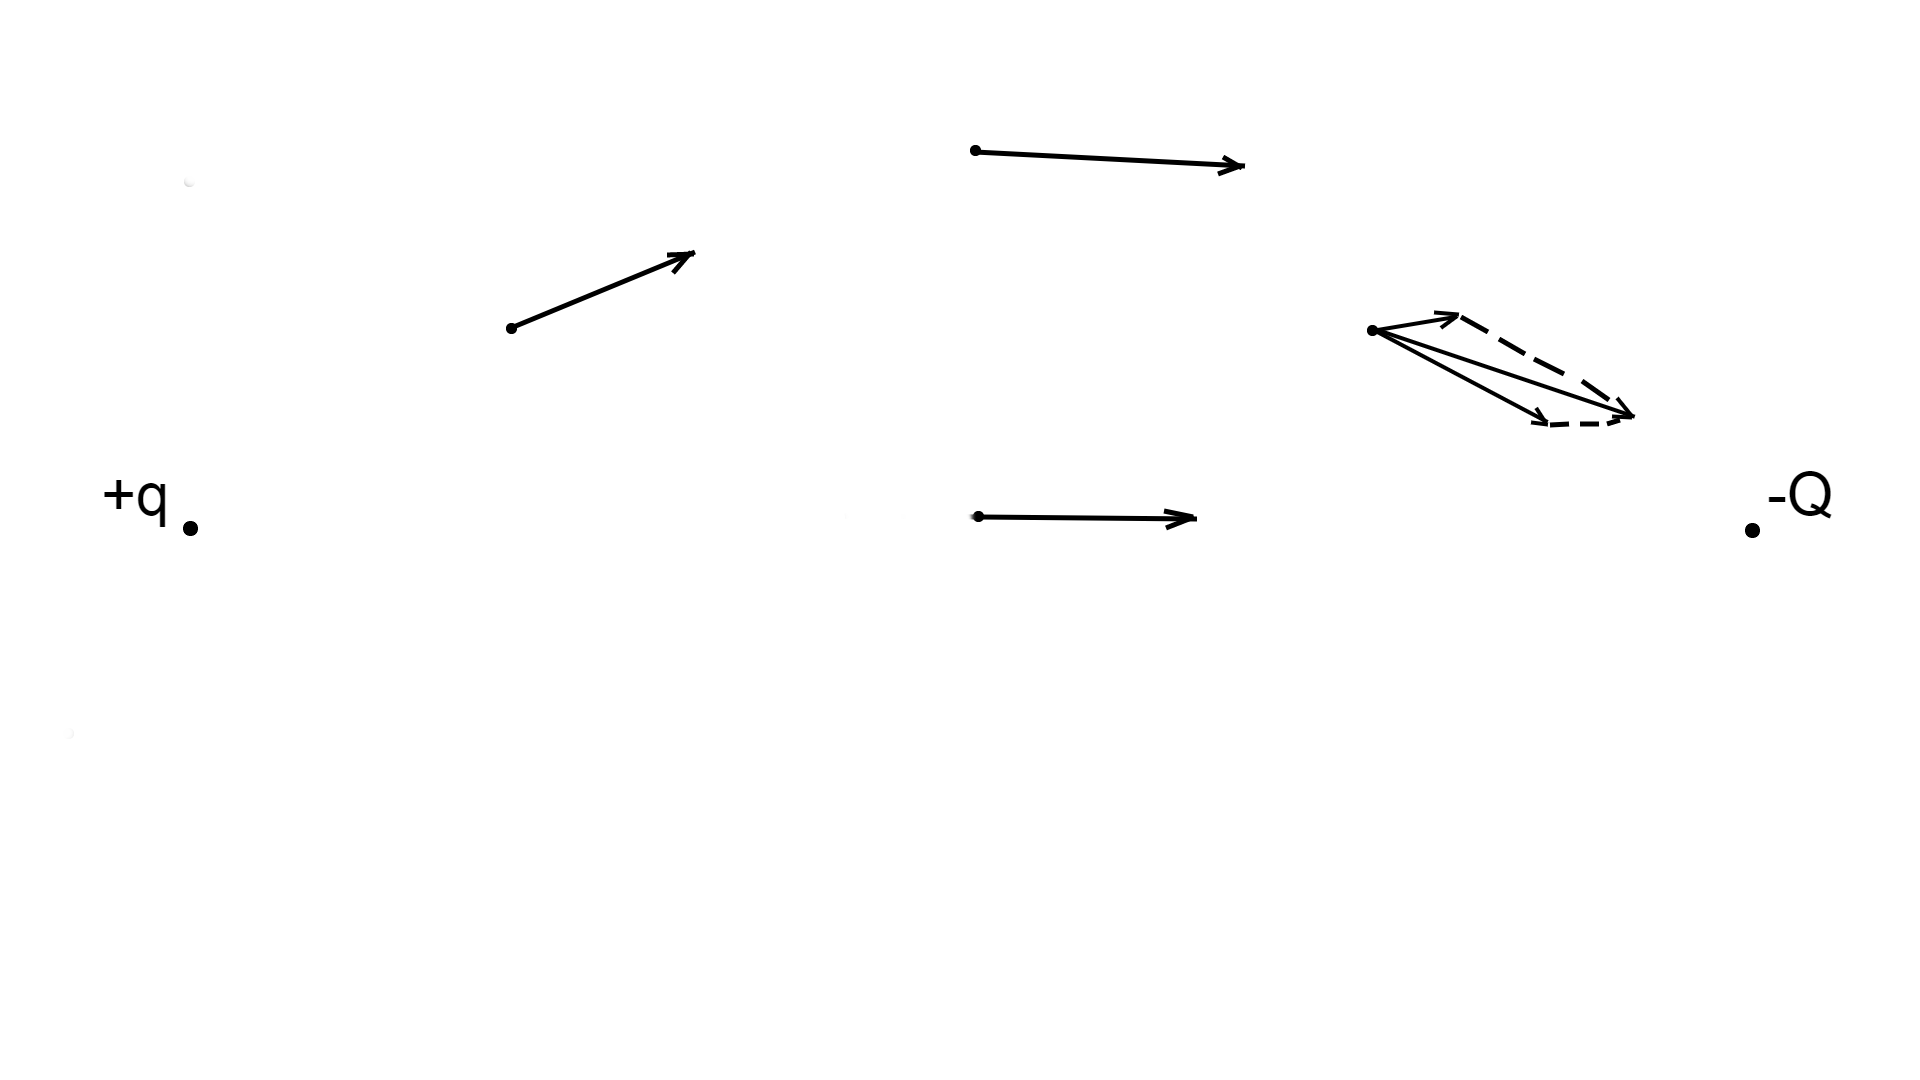
\includegraphics[scale=0.15]{1_1_6_5-1.png}
                %1_1_6_5-1

                Если расписать все такие силы для каждой точки пространства, получим картину(для наглядности изображены только несколько линий):
                
                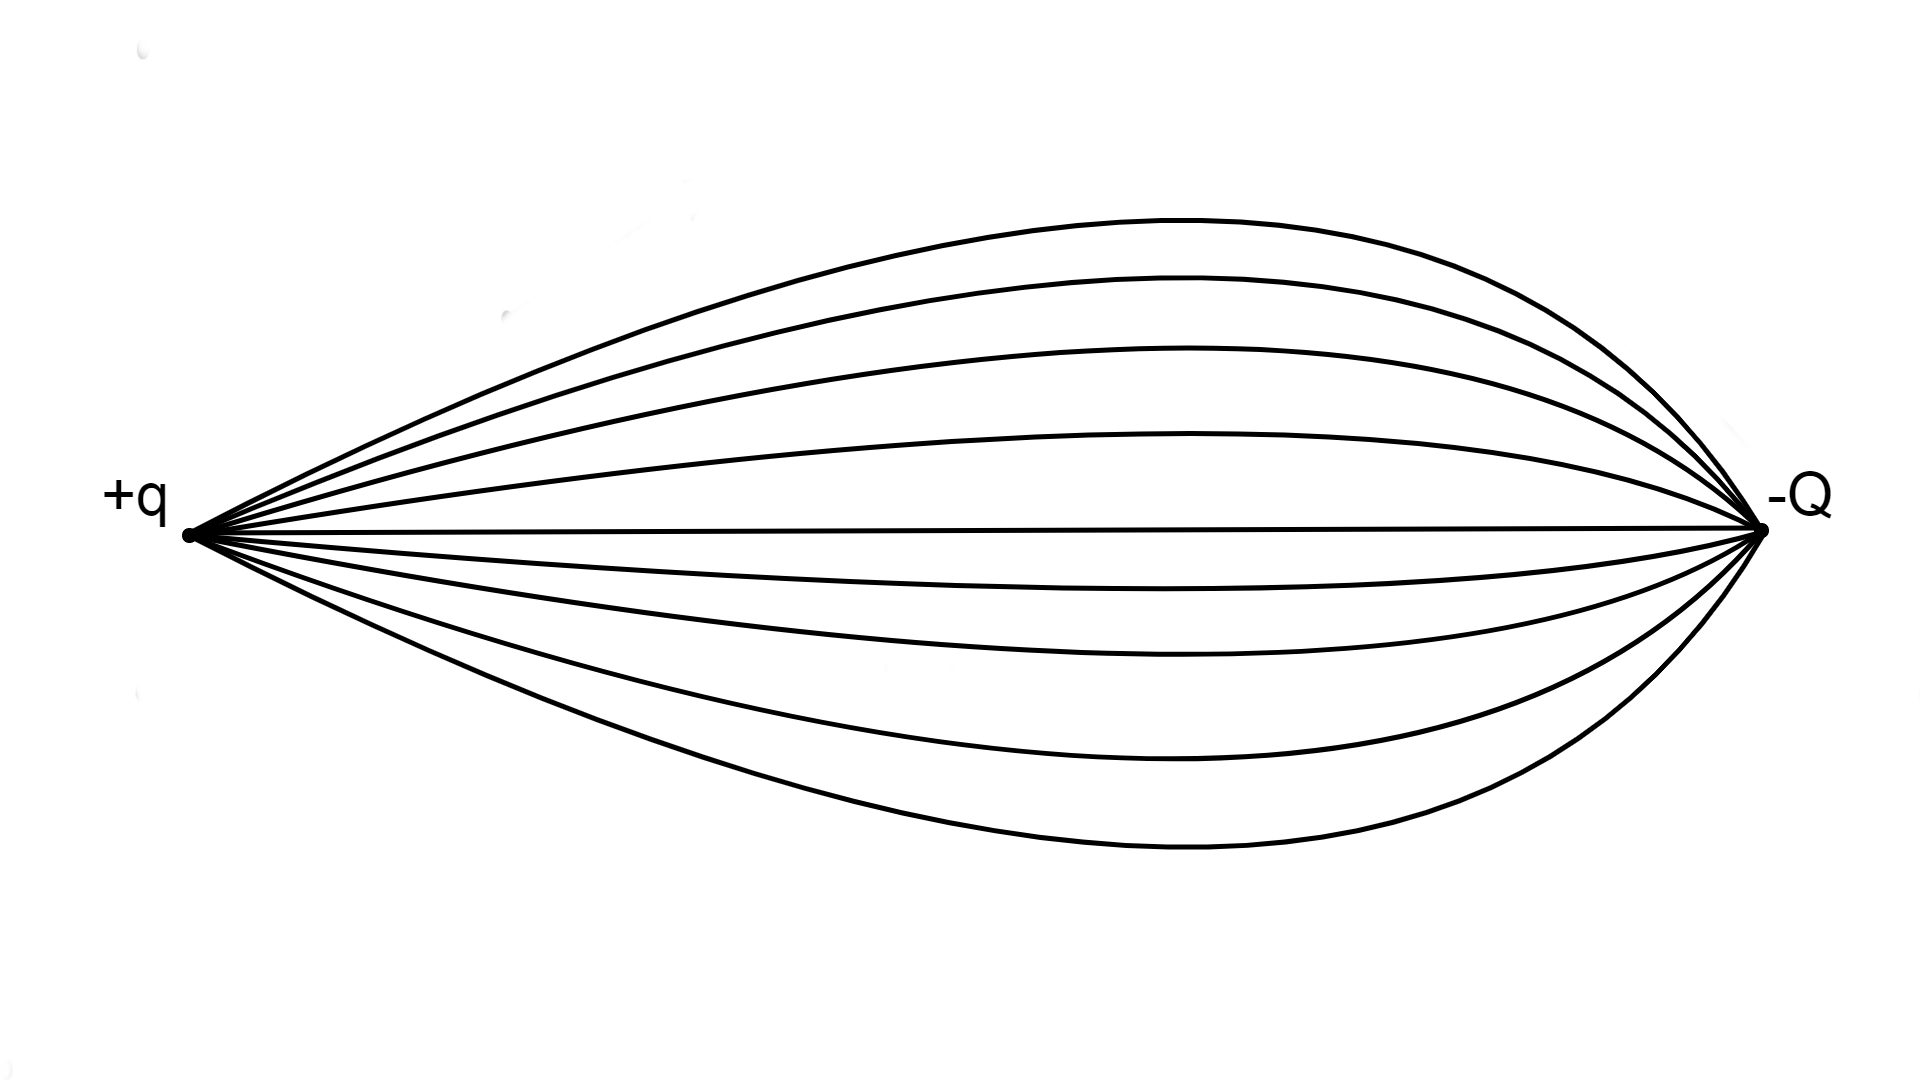
\includegraphics[scale=0.15]{1_1_6_5-2.png}
                %1_1_6_5-2

                Это и есть силовые линии.

                Силовые линии направлены от положительных к отрицательным зарядам. Положительные заряды в поле движутся по направлению силовых линий, отрицательные --- против.
        \subsubsection{Диэлектрики.}
                Диэлектрики(изоляторы) --- вещества, имеющие свойства поляризоваться.
            \paragraph{Диэлектрики в электрическом поле.}
                В электрическом поле диэлектрики поляризуются, засчёт чего происходит ослабление поля внутри диэлектрика.
            \paragraph{Условия на границе двух диэлектриков.}
                %TODO
            \paragraph{Вектор электрической индукции.}
                Вектором электрической индукции называется \(\vec D = \varepsilon \varepsilon_0 \vec E\)
        \subsubsection{Поток вектора напряженности электрического поля.}
                Потоком вектора напряжённости электрического поля называют \(\Phi = \vec S \vec E\), где \(\vec S\) --- вектор площади, по направлению перпендикулярный плоскости.
        \subsubsection{Теорема Гаусса.}
                Поток вектора электростатической индукции поля через произвольную замкнутую поверхность равен алгебраической сумме зарядов, расположенных внутри этой поверхности.
                
                \(\oint{\vec D d\vec S} = \sum{q_i}\)
        \subsubsection{Напряженность электрического поля в простейших системах.}
            \paragraph{Точечный заряд.}
                \(E = k\frac{q}{l^2}\)
            \paragraph{Система точечных зарядов.}
                \(\vec E = \sum{(k\frac{q_i}{l_i^2} \cdot \frac{\vec{l_i}}{l_i})}\)
            \paragraph{Однородно заряженная плоскость.}
                Произвольная плоскость: \(E_\perp = k \sigma \Omega\)

                Для \(\infty\) плоскости: \(E = 2\pi k \sigma\)
            \paragraph{Однородно заряженная сфера.}
                \(l < R\): 
                
                По т. Гаусса, \(\varepsilon \varepsilon_0 E S = \sum{q_i} = 0\)(т.к. внутри нет зарядов)

                \(E = 0\)

                \(l > R\): 
                
                По т. Гаусса, \(\varepsilon \varepsilon_0 E S = \sum{q_i} = q\)
                
                \(\varepsilon \varepsilon_0 E \cdot 4\pi l^2 = q\)

                \(E = \frac{q}{4\pi \varepsilon \varepsilon_0 l^2} = k\frac{q}{l^2}\)

                Для \(l = R\) можно представить и так, и так, по ситуации.
            \paragraph{Однородно заряженный шар.}
                \(E = k\frac{q}{l^2}\)

                Для центра(\(l = 0\)): \(E = 0\)
        \subsubsection{Силовое воздействие электрического поля на поверхность (давление).}
                Для равномерно заряженной поверхности, с одной стороны которой поле равно \(E_2\), с другой --- \(E_1\), 
                
                Ограничим поверхность цилиндром площадью сечения \(S\).

                По т. Гаусса: \(\varepsilon\varepsilon_0 E_2 S - \varepsilon\varepsilon_0 E_1 S = S\sigma\).
                
                \(\sigma = \varepsilon\varepsilon_0(E_2 - E_1)\)

                Пусть поверхность создаёт некоторое поле \(E_\sigma\). Выразим \(E_2 = E_0 + E_\sigma\), а \(E_1 = E_0 - E_\sigma\)

                \(P = \frac{\sigma S E_0}{S} = \varepsilon\varepsilon_0 E_0(E_2 - E_1)\)

                \(\begin{cases}
                        E_1 = E_0 - 2\pi k \sigma\\
                        E_2 = E_0 + 2\pi k \sigma
                    \end{cases} \Rightarrow E_0 = \frac{E_1+E_2}{2}\)

                \(P = \varepsilon\varepsilon_0 \frac{E_1 + E_2}{2}(E_2 - E_1) = \frac{E_2^2}{8\pi k} - \frac{E_1^2}{8\pi k}\)
        \subsubsection{Потенциальность электростатического поля.}
            \paragraph{Работа по замкнутому контуру в электростатическом поле.}
                Работа по замкнутому контуру в электростатическом поле, в отличие от электрического, \(A = 0\).
            \paragraph{Потенциал электрического поля.}
                Потенциальной энергией \(W\) электростатического поля в точке называется работа по принесению пробного заряда из \(\infty\) в данную точку(при условии, что кинетическая энергия при этом была равна \(0\)).

                Потенциалом назовём отношение потенциальной энергии к этому пробному заряду: \(\varphi = \frac{W}{\Delta q}\).
            \paragraph{Разность потенциалов.}
                Разность потенциалов двух точек \(\phi_1 - \phi_2 = -\vec E l = U_{12}\) --- напряжение между точками 1 и 2.
            \paragraph{Потенциал электрического поля в простейших системах.}
                \textbf{Точечный заряд.}
                
                \(W = A = -\int_\infty^{r_0} \Delta q\frac{kQ}{r^2} \cdot dr = k\frac{\Delta q Q}{r_0}\)

                \(\varphi = \frac{W}{\Delta q} = k\frac{Q}{r_0}\)

                \textbf{Система точечных зарядов.}
                
                \(\varphi = \sum{\phi_i}\)

                \textbf{Заряженное кольцо (на оси).}

                \(\varphi = \int k\frac{dq}{\sqrt{R^2 + l^2}} = k\frac{q}{\sqrt{R^2 + l^2}}\), где \(R\) --- радиус кольца, \(l\) --- расстояние до центра кольца.

                \textbf{Однородно заряженная сфера.}
                
                \(l \leq R\): \(\varphi = k\frac{q}{R}\)

                \(l \geq R\): \(\varphi = k\frac{q}{l}\)

                В присутствии заряда \(Q\) на расстоянии \(l\) от центра сферы, в любой точке внутри сферы:

                \(\varphi = k(\frac{q}{R} + \frac{Q}{l})\)
            \paragraph{Эквипотенциальные поверхности.}
                Эквипотенциальными поверхностями называются поверхности, в любой точке которых потенциал одинаков.
            \paragraph{Силы изображения.}
                %TODO
            \paragraph{Заземление.}
                Заземлением проводника называется его соединение с точкой или объектом, поддерживающим нулевой потенциал. То есть объект способен отдавать и забирать любое количество зарядов таким образом, что потенциал проводника равняется нулю.
        \subsubsection{Энергия электрического поля и обусловленная электрическим полем.}
            \paragraph{Энергия точечного заряда в электрическом поле.}
                %TODO
            \paragraph{Плотность энергии электрического поля.}
                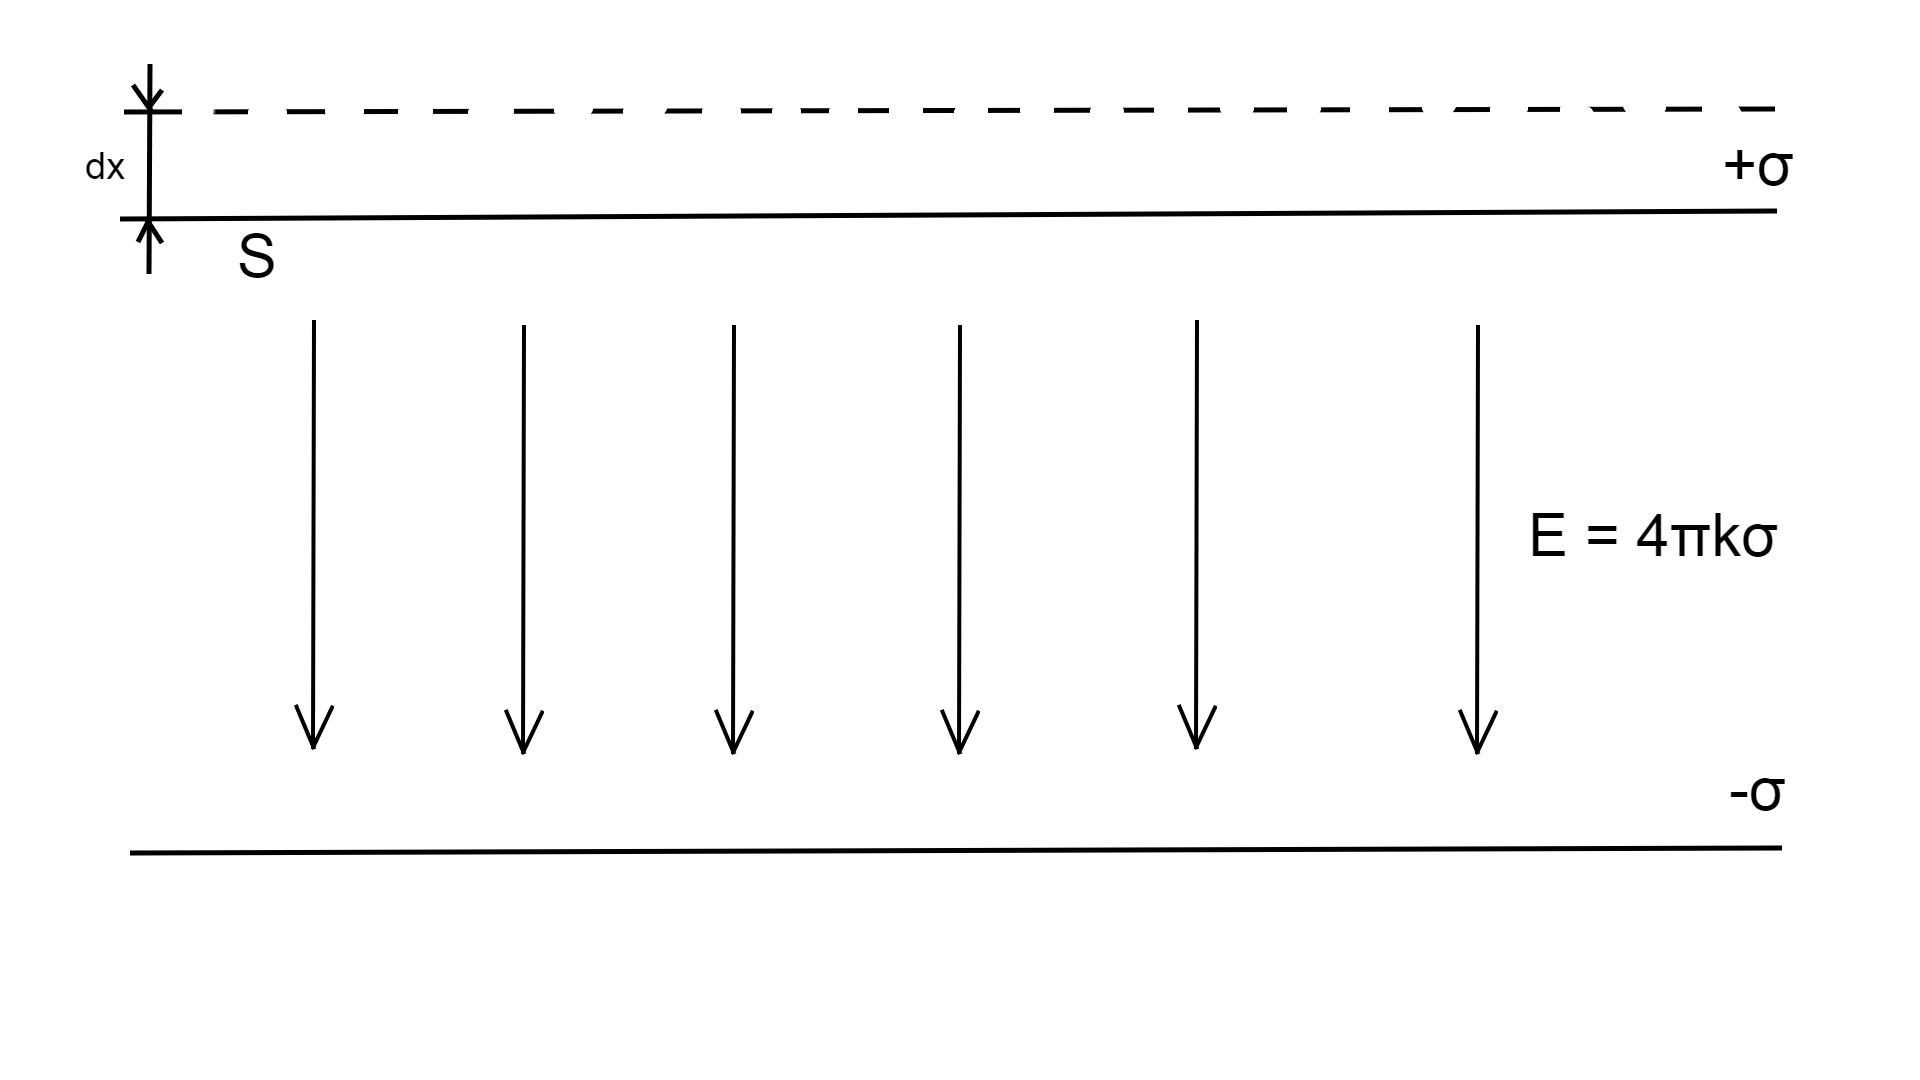
\includegraphics[scale=0.15]{1_1_13_2-1.png}    

                %1_1_13_2-1
                \(dA = 2\pi k \sigma^2 S dx = \frac{E^2}{8\pi k} \cdot S dx\)

                \(\rho_E = \frac{E^2}{8\pi k}\)
            \paragraph{Энергия взаимодействия точечных зарядов.}
                \(W = q_2\phi_1 = k\frac{q_1q_2}{l}\)

                \(W = \frac{\sum{q_i\phi_i}}{2}\)
            \paragraph{Энергия взаимодействия сложных электрических систем.}
                \(\rho_E = \frac{(\vec{E_1} + \vec{E_2})^2}{8\pi k} = \frac{E_1^2}{8\pi k} + \frac{E_2^2}{8\pi k} + (\frac{2\vec{E_1}\vec{E_2}}{8\pi k})\)

                \(W = \frac{2\vec{E_1}\vec{E_2}}{8\pi k}\)
            \paragraph{Энергия заряженной сферы.}
                \(dA = dW = \varphi \cdot dq = k\frac{q}{R}\cdot dq\)

                \(W = \int{k\frac{q}{R}\cdot dq} = k\frac{q^2}{2R}\)
        \subsubsection{Проводники в электрическом поле.}
            \paragraph{Экранирование.}
                Часть пространства, обнесённая заземлённым проводником называется экранированной. В экраннированной области \(\varphi\) --- \(const\).
            \paragraph{Метод электростатических изображений.}
                Метод изображений --- метод, применяющийся при решении задач-систем заряд-проводник. Его суть заключается в том, чтобы расставить заряды-``изображения'' таким образом, что электростатическое поле на границе проводника было равно нулю, а сила взаимодействия заряда и проводника равнялась силе взаимодействия заряда и его ``изображений''.
            \paragraph{Равновесие зарядов на проводниках и энергия.}
                %TODO
        \subsubsection{Электрическая емкость.}
            \paragraph{Конденсатор.}
                Конденсатор --- система, предназначенная для накопления электрического поля и заряда.
            \paragraph{Связь емкости, напряжения и заряда на конденсаторе.}
                \(Q = CU\)
            \paragraph{Расчет емкости плоского конденсатора.}
                \(U = 4\pi k\sigma d = 4\pi k \frac{Q}{S}d\)

                \(Q = \frac{US}{4\pi kd} = U(\frac{\varepsilon\varepsilon_0 S}{d}) = UC\)
            \paragraph{Расчет емкости простых конденсаторов (сфера, цилиндр).}
                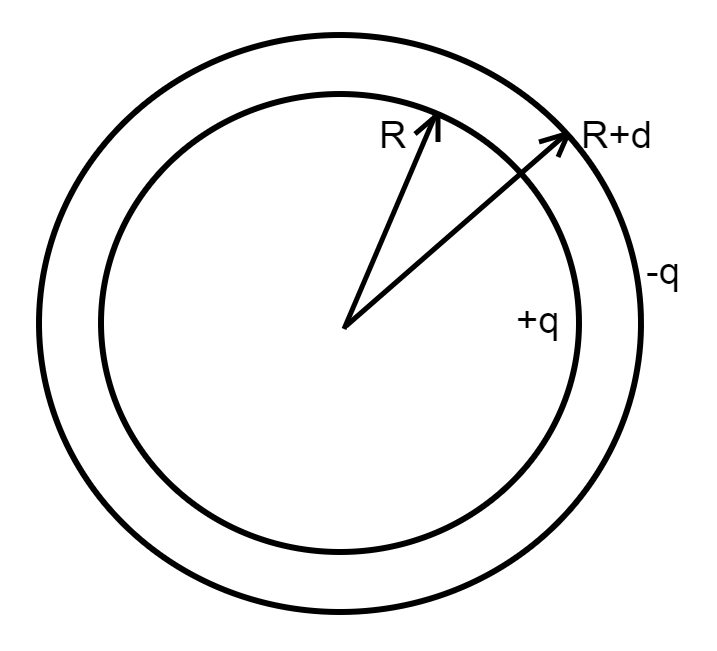
\includegraphics[scale=0.2]{1_1_15_4-1.png}

                %1_1_15_4
                \(\abs{\Delta \varphi} = \abs{k\frac{q}{R} - k\frac{q}{R+d}} = \abs{\frac{kqR+kqd-kqR}{R(R+d)}}\)

                \(C = \frac{R(R+d)}{k\cdot d}\)

                При \(d\to\infty\), \(C = \frac{R}{k}\)
            \paragraph{Составные емкости.}
                \textbf{Последовательное соединение емкостей.}
                    
                \(\frac{1}{C} = \sum{\frac{1}{C_i}}\)

                \textbf{Параллельное соединение емкостей.}
                
                \(C = \sum{C_i}\)

                \textbf{Емкостные цепи.}
                %TODO
                \textbf{Симметричные и несимметричные емкостные цепи.}
                %TODO
            \paragraph{Реальные системы емкостей.}
                %TODO
            \paragraph{Энергия электрического поля конденсатора.}
                \(W = \frac{CU^2}{2}\)
        \subsection{Электродинамика.}
        \subsubsection{Постоянный электрический ток.}
            \paragraph{Сила тока.}
                \(I = \frac{dq}{dt}\)
            \paragraph{Плотность электрического тока.}
                \(j = \frac{I}{S} = nev\)
        \subsubsection{Электрическое сопротивление.}
            \paragraph{Удельное сопротивление и удельная электропроводность (проводимость).}
                Удельное сопротивление --- характеристика материала, из которого сделан элемент сопротивления, обозначается \(\rho\). Обратная величина --- \(\sigma = \frac{1}{\rho}\)(проводимость).
                
            \paragraph{Выражение сопротивления через удельное сопротивление.}
                \(R = \rho\frac{l}{S}\)
        \subsubsection{Напряжение.}
            \paragraph{Падение напряжения и разность потенциалов.}
                Разность потенциалов возникает на конденсаторах и на элементах цепи, имеющих сопротивление.
        \subsubsection{Закон Ома.}
                \(I = \frac{U}{R}\)
        \subsubsection{Амперметр и вольтметр.}
            \paragraph{Идеальный амперметр.}
                Амперметр измеряет силу тока. Идеальный амперметр не имеет сопротивления.
            \paragraph{Идеальный вольтметр.}
                Вольтметр измеряет напряжение между клеммами. Идеальный вольтметр не имеет сопротивления.
            \paragraph{Реальные амперметр и вольтметр.}
                Реальные приборы имеют собственное внутреннее сопротивление.
        \subsubsection{Составные сопротивления.}
            \paragraph{Последовательное соединение проводников.}
                \(R = \sum{R_i}\)
            \paragraph{Параллельное соединение проводников.}
                \(\frac{1}{R} = \sum{\frac{1}{R_i}}\)
            \paragraph{Цепи сопротивлений, смешанное соединение проводников.}
                %TODO
            \paragraph{Симметричные и несимметричные цепи сопротивлений.}
                %TODO
        \subsubsection{Электродвижущая сила (ЭДС).}
                ЭДС --- величина напряжения, на которое источник тока или напряжения поднимает потенциал между его клеммами. Обозначается \(\varepsilon\).
            \paragraph{Внутреннее сопротивление источника тока.}
                Внутреннее сопротивление источника --- элемент сопротивления, содержащийся в источнике. К цепи подключается последовательно.
        \subsubsection{Закон Ома для участка цепи.}
                \(I = \frac{U}{R}\)
        \subsubsection{Закон Ома для полной электрической цепи.}
                \(I = \frac{\varepsilon}{R + r}\)
        \subsubsection{Источник напряжения и источник тока.}
                Источник тока поддерживает постоянную силу тока.

                Источник напряжения поддерживает постоянную ЭДС.
        \subsubsection{Гальванометр.}
                Гальванометр --- прибор, измеряющий прохошедший через него заряд.
        \subsubsection{Правила Кирхгофа.}
            \paragraph{Падение напряжения на сопротивлении, емкости и вольтметре.}
                Падение напряжения на сопротивлении и ёмкости имеет разную природу. На ёмкости --- электростатическую, а на сопротивлении --- в следствии закона Ома.
            \paragraph{Первое правило Кирхгофа.}
                Алгебраическая сумма токов, сходящаяся в любом узле цепи, равна нулю.
                
                \(\sum{I_i} = 0\)
            \paragraph{Второе правило Кирхгофа.}
                В замкнутом контуре алгебраическая сумма ЭДС равна алгебраической сумме падений напряжений.

                \(\sum{\varepsilon_i} = \sum{I_iR_i}\)
            \paragraph{Закон сохранения заряда в узлах с конденсаторами.}
                %TODO
            \paragraph{Переходные процессы, зарядка и разрядка конденсатора через сопротивление, время переходного процесса (RC).}
                Переходные процессы — процессы, возникающие в электрических цепях при различных воздействиях, приводящих их из стационарного состояния в новое стационарное состояние.

                Зарядка и разрядка конденсаторов через споротивление происходит с потерей энергии --- выделением тепла.

                %TODO
        \subsubsection{Закон изменения энергии в электрических цепях.}
            \paragraph{Работа ЭДС.}
                \(A = q\varepsilon\)(\(q\) --- перенесённый заряд).
            \paragraph{Работа электрического тока.}
                \(A = UIt\)
            \paragraph{Мощность электрического тока.}
                \(P = UI\)
            \paragraph{Закон Джоуля-Ленца.}
                \(Q = I^2Rt\)
        \subsubsection{Полупроводники.}
            \paragraph{Полупроводниковый диод.}
                Диод --- элемент, который работает как ключ, пропускающий ток только в одну сторону, причём только при определённой силе тока.
            \paragraph{Цепи с полупроводниковыми диодами.}
        \subsubsection{Электрический ток в неметаллах.}
            \paragraph{Электрический ток в электролите.}
            \paragraph{Электролиз.}
            \paragraph{Электрический ток в вакууме.}
        \subsubsection{Электровакуумные приборы.}
    
\end{document}